\begin{blocksection}
\question
Consider the following code segment:
\begin{verbatim}
Loop:	lw    t1, 0(t2)
		srl   t1, t1, 16
		sw    t1, 0(t2)
		addi  t2, t2, -4
		sub	  t4, t3, t2
		bne   t4, 0, Loop
End: 	sll   x0, x0, x0
\end{verbatim}
Assume that originally \texttt{t3 = t2 - 196}.

Assume a standard 5 stage pipeline with no forwarding. Register file writes happen before reads, in the same clock cycle. Comparator logic begins at the end of the decode stage. We do not have a branch delay slot. Fill in the corresponding pipeline stages (F, D, E, M, W) at the appropriate times in the table below. 

If the instruction requires a stall, write the stage again in the table. For example, if an instruction starts at cycle 2 but needs two stalls for the execute stage, then you would write “F D E E E M W” for cycles 2 - 8. 

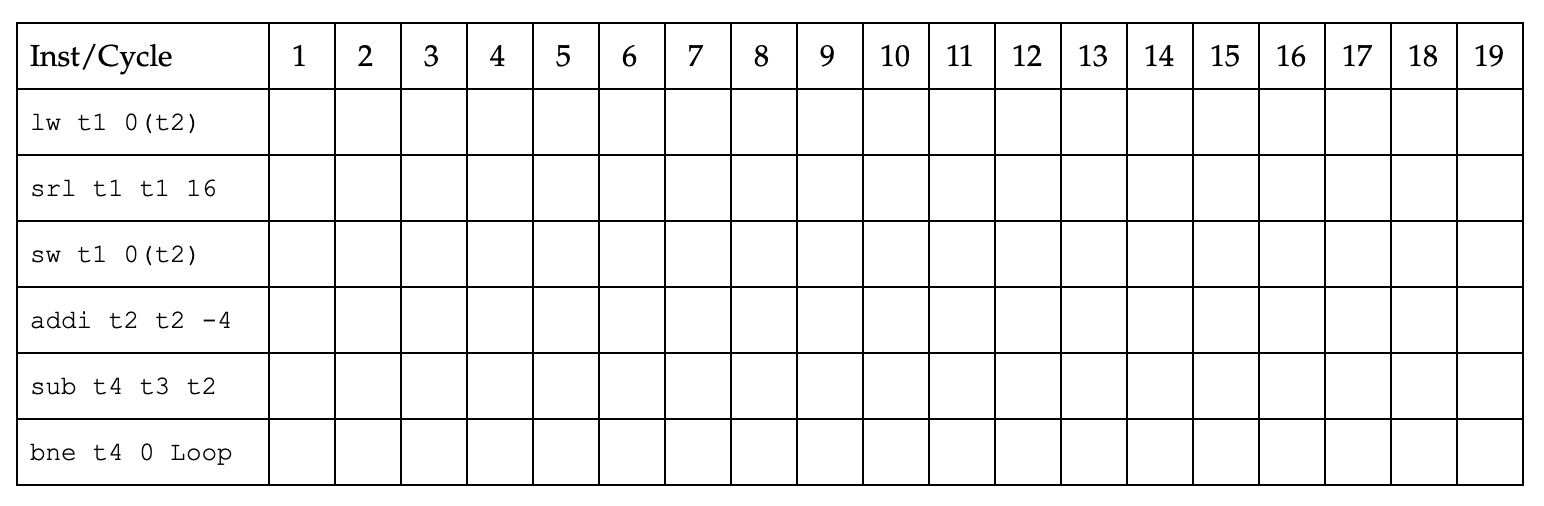
\includegraphics[width=\textwidth]{datapath/pipelining_hard}

\begin{solution}
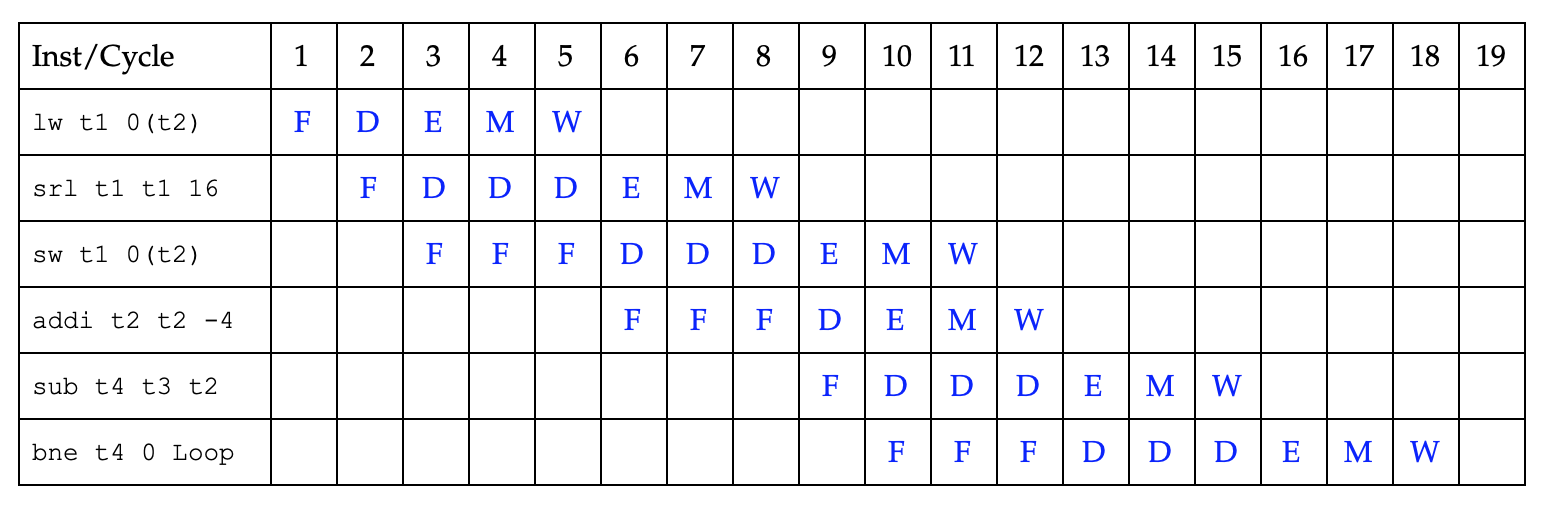
\includegraphics[width=\textwidth]{datapath/pipelining_hard_sol}
\end{solution}

\end{blocksection}